\documentclass[dvipdfmx,8pt]{beamer}
\usepackage{bxdpx-beamer} % dvipdfmxなので必要
\usepackage{pxjahyper} % 日本語のしおり用
% \usepackage{minijs} % フォントの設定?pLaTeX, upLaTaXなら不要

\usepackage{url} % 文中にリンク張る用
\usepackage{comment} % 複数行コメントアウト用
\usepackage{amsmath} %数式用
\renewcommand{\kanjifamilydefault}{\gtdefault} % 既定をゴシック体に変更

\newcommand{\probability}[1]{\mathrm{Pr}[{#1}]}

% \usetheme{metropolis}
\AtBeginSection{\frame{\sectionpage}} % Section毎に見出しを追加

\title{The Elements of Statistical Learning\\Chap.18: High-Dimensional Problems: $p \gg N$}
\date{\today}
\author{Kosuke Kito}

\begin{document}
  \maketitle
  \begin{frame}{本日のお題 - $p \gg N$ 問題}
    特徴量の数がサンプル数よりもずっと大きいとき($p \gg N$)に困っちゃう話.
    \begin{itemize}
      \item 困っちゃうポイントは, high variance と overfitting
      \item simple, highly regularized な手法が使われる.
      \item 主な話題は以下の2つ.
      \begin{itemize}
        \item prediction
        \item feature selection, assesment
      \end{itemize}
    \end{itemize}
    \begin{figure}[htb]
      \centering
      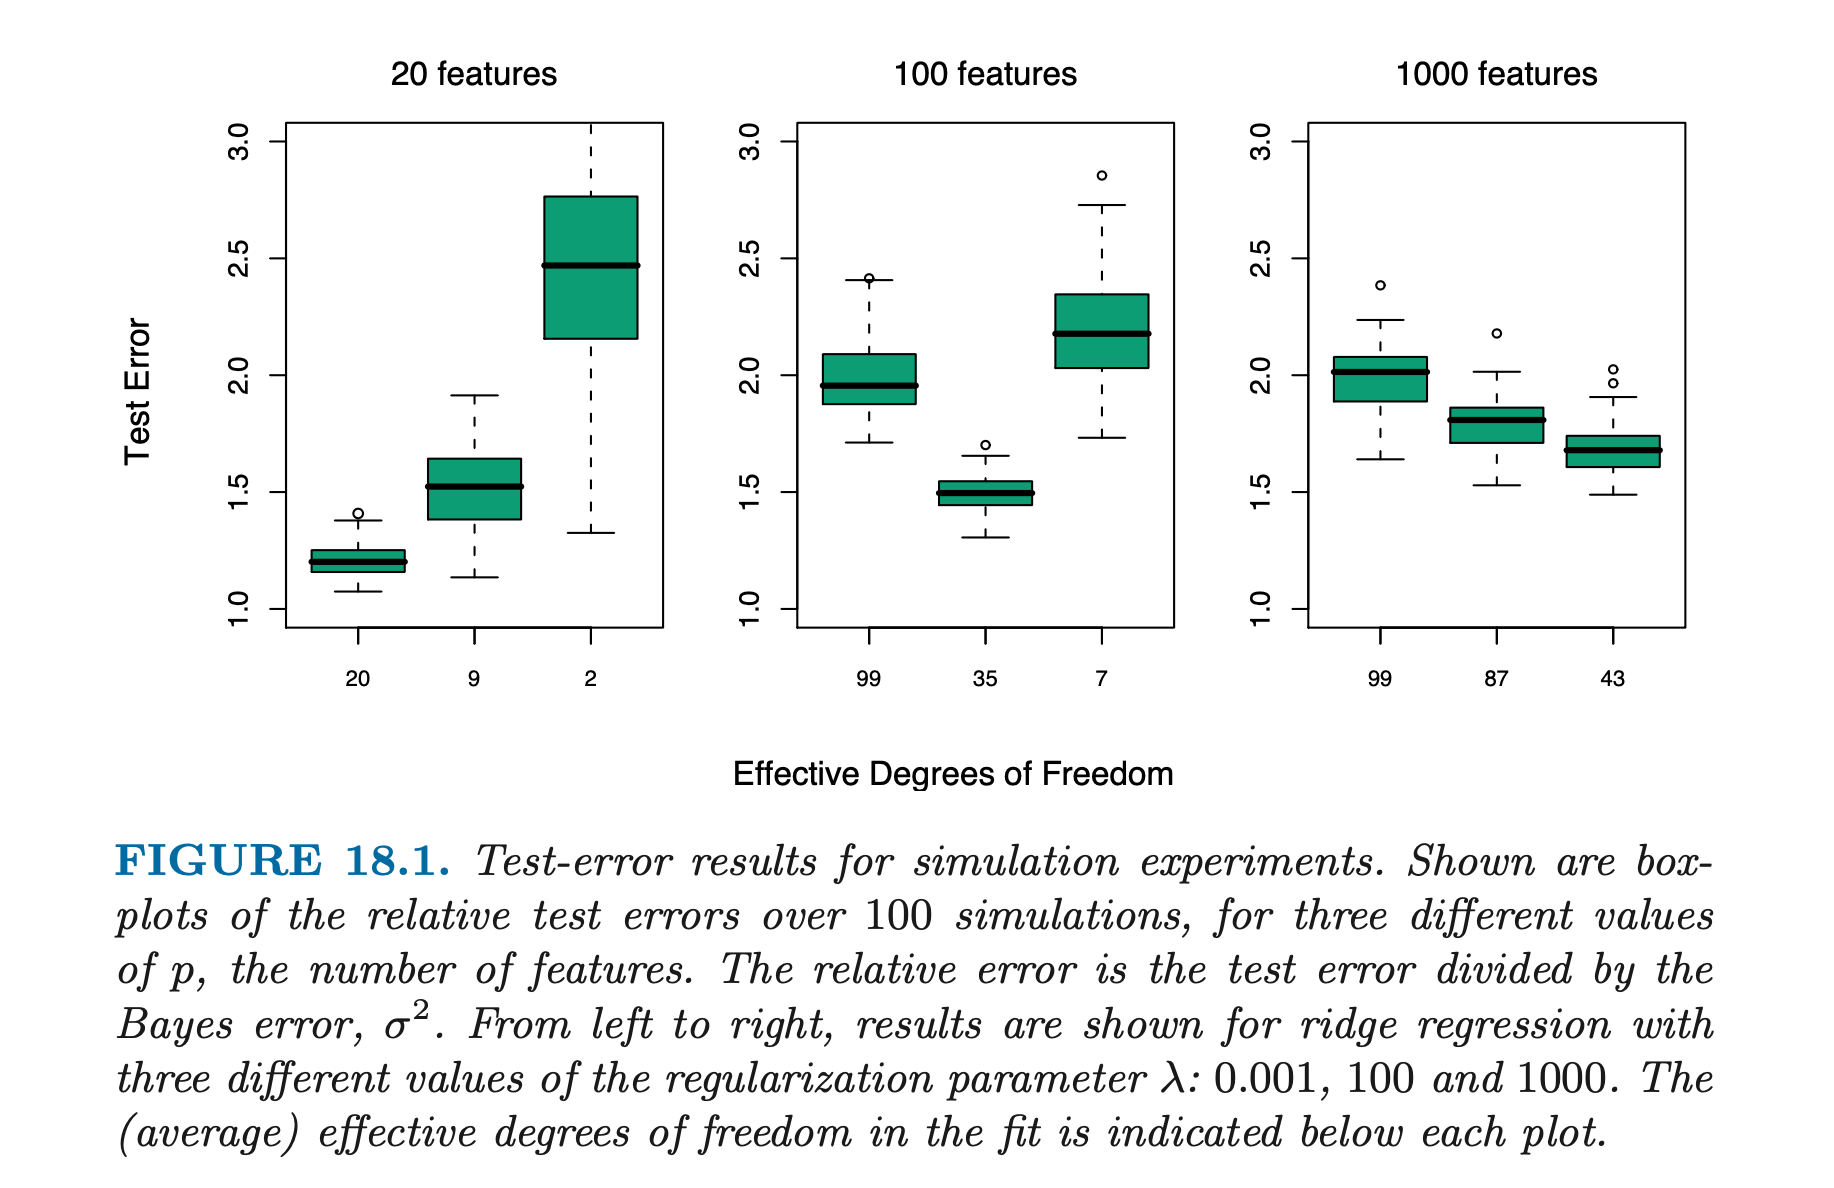
\includegraphics[width=5cm]{./images/test-error-in-high-demension.png}
    \end{figure}
  \end{frame}
  \begin{frame}{流れ}
    \begin{itemize}
      \item 流れを書く.
    \end{itemize}
  \end{frame}
  \section{}
  \begin{frame}{LDAの復習1 - コンセプト}
    $p\gg N$問題の最初の回避策は, ``Diagonal LDA''という線型判別法の強烈な正規化バージョン.

    とりあえず, LDAの復習. (不要であれば飛ばします. )
    \begin{itemize}
      \item 分類のための手法.
      \item 各入力$x$に対して, 事後確率$\probability{k \mid X=x}$が最大になるクラス$k$をクラスの推定値とする.
      \item 各クラス内で, 入力変数は多変量ガウス分布に従うと仮定.
      \item 各クラスのクラス内分散が等しいと仮定. \\
        →クラス間の境界が線形になる.
      \item 数式で書くと次ページの流れ.
    \end{itemize}
  \end{frame}
  \begin{frame}{LDAの復習2 - 定式化と計算}
    \begin{itemize}
      \item 各クラス内の分布はガウス分布と仮定.
        \[
          \probability{X=x | G=k}=\frac{1}{(2 \pi)^{\frac{p}{2}}|\Sigma|^{\frac{1}{2}}}e^{-\frac{1}{2}(x-\mu_k)^\mathrm{T}\Sigma(x-\mu_k)}
        \]
      \item ベイズの定理より事後確率は以下.
        \[
          \probability{k \mid X=x}=\frac{\probability{X=x | G=k}\probability{G=k}}{\sum_l\probability{X=x | G=l}\probability{G=l}}
        \]
      \item 事後確率の大小比較のため対数比(log-ratio)を見る.
        \begin{eqnarray*}
          \log \frac{\probability{k \mid X=x}}{\probability{l \mid X=x}} &=& \log \frac{\pi_k}{\pi_l}-\frac{1}{2}(\mu_k+\mu_l)^{\mathrm{T}}\Sigma^{-1}(\mu_k-\mu_l)+x^{\mathrm{T}}\Sigma^{-1}(\mu_k-\mu_l) \\
          &=& (\log\pi_k - \frac{1}{2}\mu_k^{\mathrm{T}}\Sigma^{-1}\mu_k+x^{\mathrm{T}}\Sigma^{-1}\mu_k)\\
          && - (\log\pi_l - \frac{1}{2}\mu_l^{\mathrm{T}}\Sigma^{-1}\mu_l+x^{\mathrm{T}}\Sigma^{-1}\mu_l)
        \end{eqnarray*}
      \item 結局, 点$x$がクラス$k$である度合い(discriminant score)は以下を評価すれば良い.
        \[
          \delta_k(x)=x^{\mathrm{T}}\Sigma^{-1}\mu_k-\frac{1}{2}\mu_k^{\mathrm{T}}\Sigma^{-1}\mu_k+\log\pi_k
        \]
    \end{itemize}
  \end{frame}
  \begin{frame}{Diagonal LDA - 線型判別法の強烈な正規化バージョン}
    \begin{itemize}
      \item 基本的なコンセプトは, 前述のLDAと同じ. 以下の条件を追加する.
        \[
          \Sigma = \mathrm{diag}(s_1, s_2, \dots , s_p) \quad \mbox{(対角行列)}
        \]
      \item すると, discriminant scoreは, (クラスに依らない定数$-x^\mathrm{T}\Sigma^{-1}x$を足して2倍することで, )以下になる.
        \[
          \delta_k(x)=-\sum_{j=1}^p\frac{(x_j-\bar{x}_{kj})^2}{s_j^2}+2\log\pi_k
        \]
      \item この discriminant score を使って, 以下のルールで分類する.
        \[
          C(x)=\mathrm{arg}\max_l\delta_l(x)
        \]
    \end{itemize}
  \end{frame}
  \begin{frame}{Diagonal LDA - 線型判別法の強烈な正規化バージョン}
    Diagonal LDAについて何点か補足.
    \begin{itemize}
      \item discriminant score は距離に見える.\\
        →Diagonal LDA は, 適当な標準化をしたデータにおける nearest centroid 法のようにも見える.
      \item 変数間の共分散が$0$という仮定を、独立律(independent rule)ともいう。
      \item 高次元の時には、effective なことが多いらしい。
      \item この方法の欠点の一つは、特徴量選択(feature selection)ができないこと。高次元の入力の時には、一部の変数を選び出せる方法を使いたい。\\
        →もっと正規化の条件を強めるとパフォーマンスがさらに上がるらしい。
      \item 次は、特徴量選択が行われるような正規化の条件をかけたバージョンを考えます。
    \end{itemize}
  \end{frame}
  \begin{frame}{Nearest Shrunken Centroids}
    前出の Diagonal LDA = Nearest Centroid 法の centroid を縮小(shrinkage)させることで、特徴量選択を行えるようにする。
    \begin{itemize}
      \item 基本的な計算は、Diagonal LDAと一緒。
      \item discriminant score の計算に使うcentroid を単純な平均$\bar{x}_{kj}$から変える。
      \item まず、あるパラメータ$X_j$のクラス$k$内での平均$\bar{x}_{kj}$と全体での平均$\bar{x}_j$の差を標準化する。
        \begin{columns}[t]
          \begin{column}{0.1\columnwidth}
            % 文頭を揃えるためのからのカラム
          \end{column}
          \begin{column}{0.3\columnwidth}
            \[
              d_{kj}=\frac{\bar{x}_{kj}-\bar{x}_j}{m_k(s_j+s_0b)}
            \]
            ただし、各項は以下。
            \begin{align*}
              &m_k=\frac{1}{N_k}-\frac{1}{N}\colon \mbox{疑問点}\\
              &s_0=\mbox{小さな定数}\\
              &s_j\mbox{が小さい時に}d_{kj}\mbox{が大きくなりすぎないように}
            \end{align*}
          \end{column}
          \begin{column}{0.3\columnwidth}
            \begin{figure}[htb]
              \centering
              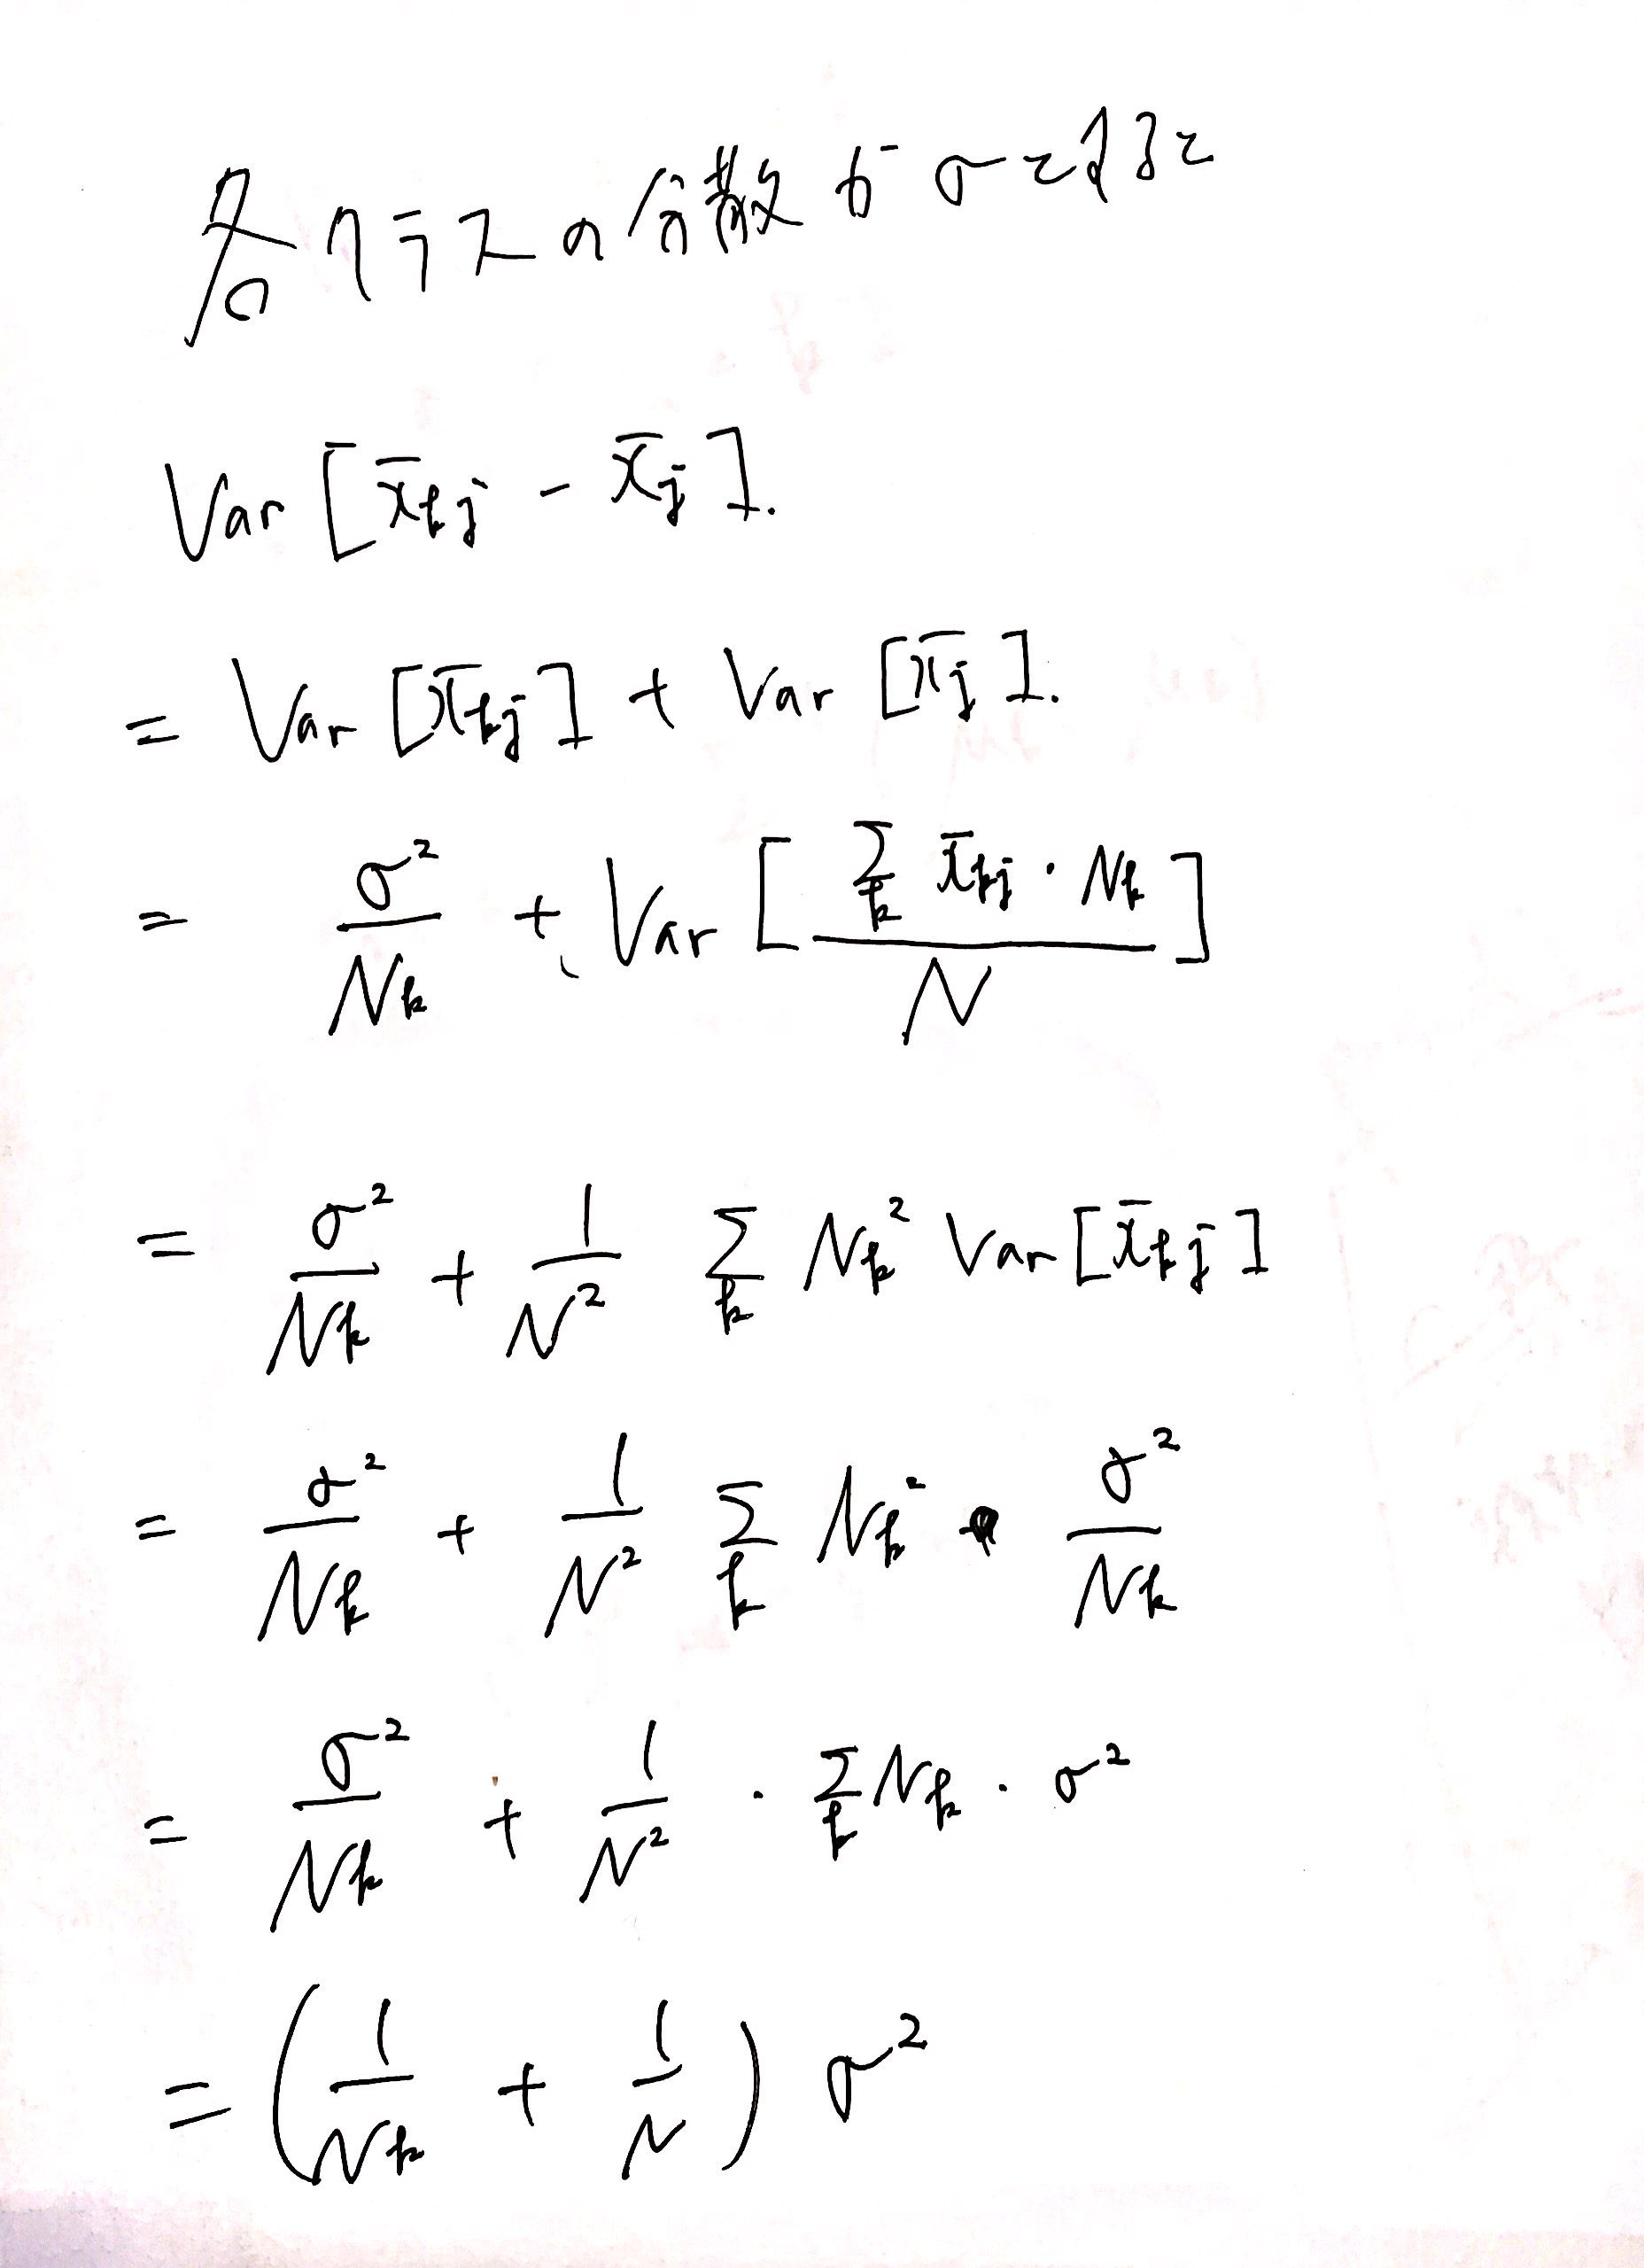
\includegraphics[width=3cm]{./images/nsc-variance-calc.jpg}
            \end{figure}
          \end{column}
        \end{columns}
    \end{itemize}
  \end{frame}
\begin{comment} % 再生核ヒルベルト空間の話を本当にするのか
  \section{再生核ヒルベルト空間\\(Reproducing Kernel Hilbert Space, RKHS)}
  \begin{frame}{今こそRKHS - カーネル法(Kernel Method)}
    \begin{itemize}
      \item RKHSは, カーネル法を実現するときに重要になる数学的な対象です.
      \item まずはカーネル法について, やりたいこととざっくり全体像の整理. \\
        \begin{itemize}
          \item 線形に分類できないもの(同心円が典型例)をうまく分類したい.
          \item 変数変換してあげると, 線形の手法を使える. \\
            \[
              (x,y) \mapsto (x^2,y^2)
            \]
          \item 高次元に写せば, ほぼ確実に線形分類可能にできる.
            \[
              (x,y)\mapsto (x,y,x^2,xy,y^2)
            \]
          \item この, 変数変換の写像を``カーネル''と呼ぶ.
          \item 一方, 高次元に写すと計算量が増える. 困る. \\
            →高次元でも計算が楽なカーネルはないものか...
          \item 正定値カーネルは内積計算が楽!内積で計算できるモデルならいい感じに使える!\\
            (SVM, CPA, etc...)
        \end{itemize}
    \end{itemize}
  \end{frame}
\end{comment}
\end{document}
